\documentclass[border=3pt]{standalone}
% Preâmbulo compartilhado pelos diagramas TikZ da aula 14 (SLAM com EIF)
\usepackage[T1]{fontenc}
\usepackage[utf8]{inputenc}
\usepackage{lmodern}
\usepackage{amsmath}
\usepackage{xcolor}
\usepackage{tikz}
\usetikzlibrary{arrows.meta,angles,quotes,decorations.pathmorphing,decorations.pathreplacing,calc,
                positioning,shapes.geometric,shapes.misc,backgrounds,fit,
                math}

% Paleta (mesma dos SVGs originais)
\definecolor{dblue}{HTML}{2A5B8C}
\definecolor{dorange}{HTML}{B3541E}
\definecolor{dgreen}{HTML}{4A7C59}
\definecolor{dred}{HTML}{9C4B4B}
\definecolor{dcream}{HTML}{F4F1EA}
\definecolor{dshade}{HTML}{DDD7C9}

% Função gaussiana (não normalizada por padrão de escala visual)
\pgfmathdeclarefunction{gauss}{3}{%
  \pgfmathparse{1/(#3*sqrt(2*pi))*exp(-((#1-#2)^2)/(2*#3^2))}%
}

% Estilos comuns (prefixo d... para não colidir com chaves internas do pgf)
\tikzset{
  >={Stealth[length=2mm]},
  dguide/.style={gray!55, dashed, line width=0.4pt},
  daxis/.style={gray!60, line width=0.7pt, ->},
  dbody/.style={fill=black!3, draw=black!80, line width=1pt},
  dacc/.style={draw=dblue, line width=1pt},
  dlbl/.style={black!55, font=\small},
  dsub/.style={black!45, font=\footnotesize},
  dstate/.style={circle, draw=black!80, fill=dcream, line width=1pt,
                 minimum size=17mm, font=\large, inner sep=1pt},
  dobs/.style={circle, draw=black!80, fill=dshade, line width=1pt,
               minimum size=14mm, font=\large, inner sep=1pt},
  dbox/.style={rounded corners=2pt, draw=black!80, fill=dcream, line width=1pt,
               align=center, inner sep=6pt},
  dop/.style={circle, draw=black!80, fill=white, line width=1pt,
              minimum size=6mm, inner sep=0pt, font=\small},
  dtrans/.style={->, dblue, line width=1pt},
  dmeas/.style={->, dorange, line width=1pt},
  dcurve/.style={line width=1pt, dblue},
  dcurveb/.style={line width=1.4pt, dorange},
}

\begin{document}
\hyphenpenalty=10000 \exhyphenpenalty=10000 \tolerance=9999 \emergencystretch=3em
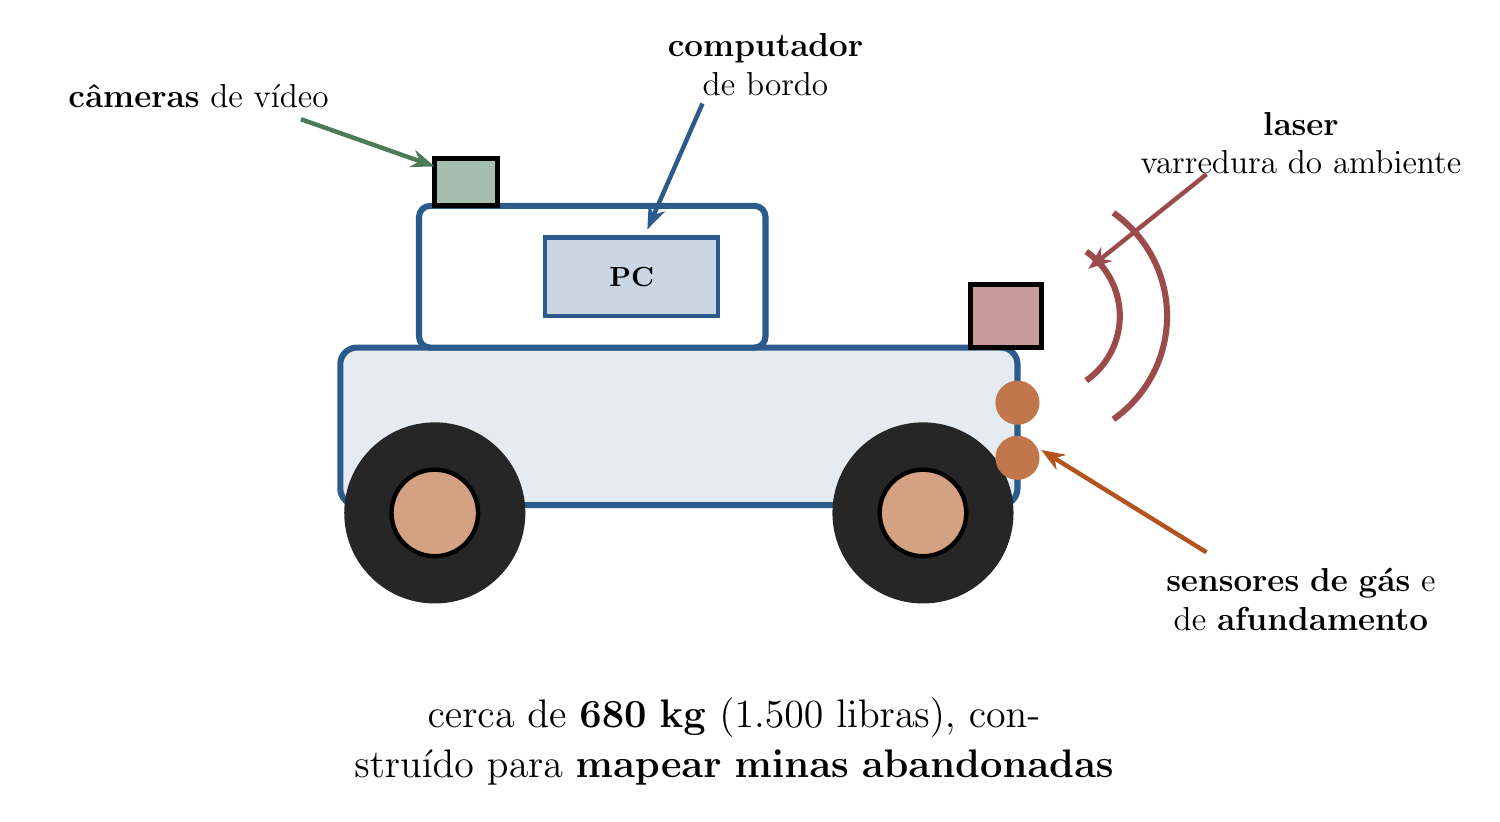
\begin{tikzpicture}[x=1cm,y=1cm]
\tikzset{t/.style={font=\large, fill=white, inner sep=2pt, text width=4.2cm, align=center},
        ar/.style={line width=1.6pt, -{Stealth[length=3mm]}}}
% chassi, cabine e rodas
\draw[line width=2.2pt, draw=dblue, fill=dblue!12, rounded corners=6pt] (4.0,3.0) rectangle (12.6,5.0);
\draw[line width=2.2pt, draw=dblue, fill=white, rounded corners=4pt] (5.0,5.0) rectangle (9.4,6.8);
\foreach \x in {5.2,11.4} {\fill[black!85] (\x,2.9) circle (1.15); \draw[fill=dorange!55, draw=black, line width=1.6pt] (\x,2.9) circle (0.55);}
% laser na frente
\draw[line width=1.8pt, fill=dred!55, draw=black] (12.0,5.0) rectangle (12.9,5.8);
\draw[dred, line width=2.2pt] (12.9,5.4) ++(-55:1.0) arc (-55:55:1.0);
\draw[dred, line width=2.2pt] (12.9,5.4) ++(-55:1.6) arc (-55:55:1.6);
% camera
\draw[line width=1.8pt, fill=dgreen!50, draw=black] (5.2,6.8) rectangle (6.0,7.4);
% sensores de gas e afundamento (frente, embaixo)
\fill[dorange!80] (12.6,3.6) circle (0.28); \fill[dorange!80] (12.6,4.3) circle (0.28);
% computador de bordo
\draw[line width=1.6pt, fill=dblue!25, draw=dblue] (6.6,5.4) rectangle (8.8,6.4); \node[font=\normalsize\bfseries] at (7.7,5.9) {PC};
% legendas
\node[t] at (16.2,7.6) {\textbf{laser}\\ varredura do ambiente};
\draw[ar, dred] (15.0,7.2) -- (13.5,6.0);
\node[t] at (2.2,8.2) {\textbf{câmeras} de vídeo};
\draw[ar, dgreen] (3.5,7.9) -- (5.2,7.3);
\node[t] at (9.4,8.6) {\textbf{computador} de bordo};
\draw[ar, dblue] (8.6,8.1) -- (7.9,6.5);
\node[t] at (16.2,1.8) {\textbf{sensores de gás} e de \textbf{afundamento}};
\draw[ar, dorange] (15.0,2.4) -- (12.9,3.7);
\node[font=\Large, text width=17cm, align=center] at (9.0,0.0) {cerca de \textbf{680 kg} (1.500 libras), construído para \textbf{mapear minas abandonadas}};
\end{tikzpicture}
\end{document}
